Find the roots of the following quadratic  equations grapically.
 \begin{multicols}{2}
\begin{enumerate}[label=\thesubsection.\arabic*,ref=\thesubsection.\theenumi, itemsep=1ex]
\item $(x-2)^2+1=2x-3$
\item $x(2x+3) = x^2+1$
\item $(x+2)^3 = x^3-4$
\item $x^2-3x-10=0$
\item $2x^2+x-6=0$
\item $ \sqrt 2x^2+7x+5 \sqrt 2=0$
\item $2x^2-x+\frac{1}{8}=0$
\item $100x^2-20x+1=0$
\item $2x^2-3x+5=0$
\item $3x^2-4 \sqrt 3x+4=0$
\item $2x^2-6x+3=0$
\item $(x+1)^2=2(x-3)$
\item $x^2-2x=(-2)(3-x)$
\item $(x-3)(2x-1)=x(x+5)$
\item $(2x-1)(x-3)=(x+5)(x-1)$
\item
$2x^2-7x+3=0$
\item
$2x^2+x-4=0$
\item
$4x^2+4\sqrt 3x+3=0$
\item
$2x^2+x+4=0$
\item
$x-\frac{1}{x}=3, x\neq{0}$
\item
$\frac{1}{x+4}-\frac{1}{x-7}=\frac{11}{30}, x\neq{-4,7}$
\item $2x^2 -5x+3 = 0$.
\item $6x^2 -x-2 = 0$.
\item $3x^2 -2\sqrt6x+2 = 0$.
\item $5x^2-6x-2 = 0$. 
\item $4x^2+3x+5 = 0$. 
\item $3x^2-5x+2 = 0$
\item $x^2+4x+5 = 0$
\item $2x^2-2\sqrt 2x+1 = 0$
\item $x+\frac{1}{x} = 3,x\neq0$
\item $\frac{1}{x}-\frac{1}{x-2} = 3, x\neq 0,2$
\item $3x^2-2x+\frac{1}{3} = 0$. 
\item $x^2-4x+3 = 0$.
\item $2x^2-4x+3 = 0$.
\end{enumerate}
\end{multicols}
Find the values of $k$ for each of the following quadratic equations, so that they have equal roots.  Verify your solution graphically.
\begin{enumerate}[label=\thesubsection.\arabic*,ref=\thesubsection.\theenumi,resume*]
\item $2x^2=kx-3=0$.
\item $kx(x-2)+6=0$.
\end{enumerate}
Represent the following situations graphically.
\begin{enumerate}[label=\thesubsection.\arabic*,ref=\thesubsection.\theenumi,resume*]
\item Janaki and Jivanti together have $45$ marbles. Both of them lost $5$ marbles each, and the product of the number of marbles they have is $124$. We would like to find out how many marbles they had to start with.
\item A cottage industry produces a certain number of toys in a day. The cost of production of each toy (in rupees) was found to be $55$ minus the number of toys produced in a day. On a particular day, the total cost of production was \rupee750. We would like to find out the number of toys produced on that day.
\item Find two numbers whose sum is $27$ and product is $182$.
\item Find two consecutive  positive integers, sum of whose squares is $365$.
\item  The altitude of a right triangle is 7 cm less than its base. If the hypotenuse is 13 cm, find the other two sides.
	\\
		\solution
		\begin{table}[h!]    
	\centering
	\begin{tabular}[12pt]{ |c| c| c|}
    \hline
    \textbf{Variable} & \textbf{Description} & \textbf{Value}\\
	\hline
	$BC$ & Hypotenuse of the triangle & 13 cm\\
	\hline
	$AB$ & Base of the triangle & $x$ cm\\
	\hline
	$AC$ & Altitude of the triangle & $x - 7$ cm\\
	\hline
\end{tabular}
	\caption{}
	\label{tab:10/4/2/5}
\end{table}
	The input parameters are available in \tabref{tab:10/4/2/5}.
Using Baudhayana's theorem,
\begin{align}
	\label{eq:10/4/2/5}
	x^2 + (x - 7)^2 &= 13^2 \\
	\implies    y = x^2 - 7x - 60 &= 0 
\end{align}
which 
 can be expressed as the conic
\begin{align}
    \vec{x}^\top\vec{V}\vec{x} + 2\vec{u}^\top\vec{x} + f = 0 \\
    \vec{V} = \myvec{1 & 0 \\ 0 & 0}, \vec{u} = \myvec{-\frac{7}{2} \\ -\frac{1}{2}}, f = -60.
\end{align}
To find the roots of 
	\eqref{eq:10/4/2/5},
we find the points of intersection of the 
conic 
with the $x$-axis 
\begin{align}
    \vec{x} = \vec{h} + k\vec{m} \\
    \vec{h} = \myvec{0 \\ 0}, \vec{m} = \myvec{1 \\ 0}
\end{align}
using
\eqref{eq:tangent_roots}. 
The values of $k$ are given by
\begin{align}
k_i    &= \frac{1}{1} \brak{\frac{7}{2} \pm \sqrt{\brak{\frac{7}{2}}^2 + 60}} \\
  \implies  k_1 &= -5, k_1 = 12
\end{align}
Hence the points of intersection are
\begin{align}
    \vec{h} + k\vec{m} = \myvec{-5 \\ 0}, \myvec{12 \\ 0}
\end{align}
See 
	\figref{fig:quad1}
Hence the solutions of 
	\eqref{eq:10/4/2/5}
are $x = -5$ and $x = 12$. We reject $x = -5$ as the length of the side
cannot be negative. Hence, the lengths of the sides are
\begin{align}
    AB = 12\ cm \,
    AC = 7\ cm \,
    BC = 13\ cm
\end{align}
See	\figref{fig:quad1}.
\begin{figure}[H]
    \centering
    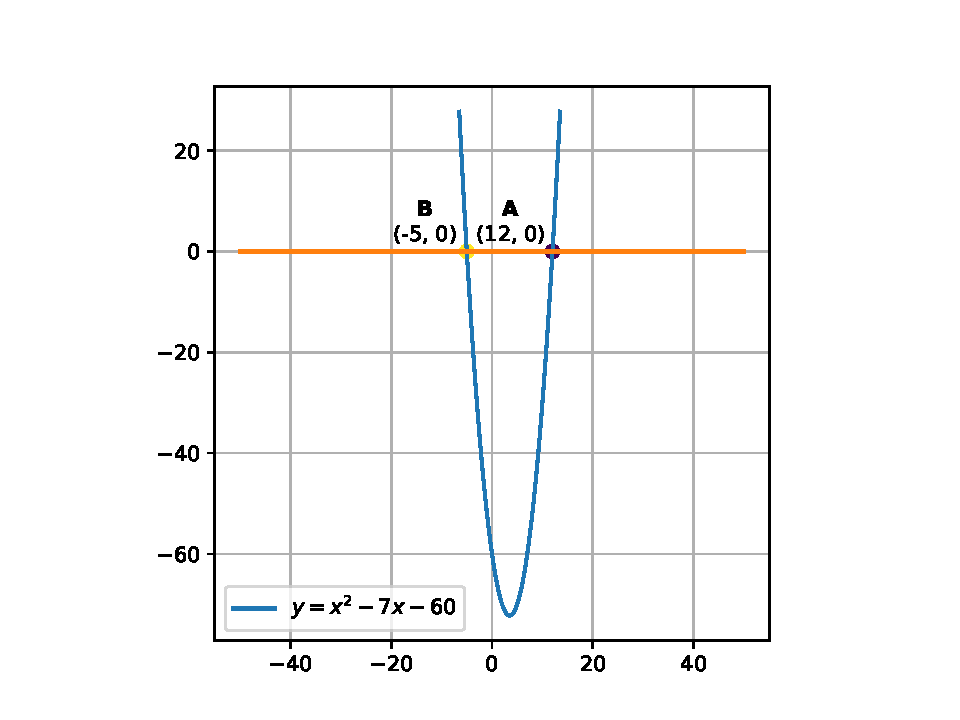
\includegraphics[width=0.75\columnwidth]{chapters/10/4/2/5/figs/parabola.pdf}
    \caption{Intersection of $y = x^2 - 7x - 60$ with the $x$-axis}
	\label{fig:quad1}
\end{figure}
%
\begin{figure}[H]
    \centering
    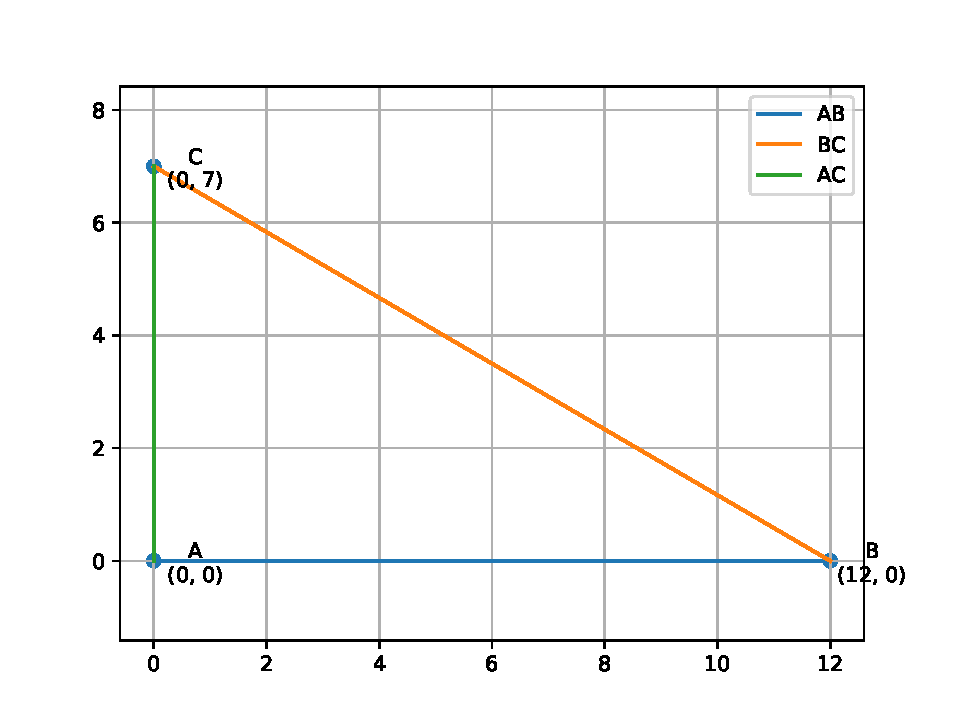
\includegraphics[width=0.75\columnwidth]{chapters/10/4/2/5/figs/triangle.pdf}
    \caption{}
	\label{fig:quad2}
\end{figure}

\item A cottage industry produces a certain number of pottery articles in a day. It was observed on a particular day that the cost of production of each article (in rupees) was $3$ more than twice the number of articles produced on that day. If the total cost of production on that day was \rupee90, find the number of articles produced and the cost of each article.
\item Is it possible to design a rectangular mango grove whose length is twice its breadth, and the area is  $800m^2$? If so, find its length and breadth.
\item Is the following situation possible? If so, determine their present ages.
\\ The sum of the ages of the two friends is 20 years. Four years ago, the product of their ages in years was $48$.
\item Is it possible to design a rectangular park of perimeter 80m and area of $400m^2$. If so, find its length and breadth.
\item The area of rectangular plot is $528m^2$. The length of the plot (in metres) is one more than twice its breadth. We need to find the length and breadth of the plot.
\item The product of two consecutive positive integers is $306$. We need to find the integers.
\item Rohan's mother is $26$ years older than him. The product of their ages (in years) $3$ years from now will be $360$. We would like to find Rohan's present age.
\item A train travels a distance of $480km$ at a unifom speed. If the speed had been $8km/h$ less, then it would have taken $3 $ hours more to cover the same distance. We need to find the speed of the train.
\item The sum of the reciprocals of Ram's ages, (in years) 3 years ago and 5 years from now is $\frac{1}{3}$. Find his present age.
\item In a class test, the sum of Shefali's  marks in Mathematics and English is $30$. Had she got $2$ marks more in Mathematics and $3$ marks less in English, the product of their marks would have been $210$. Find her marks in the two subjects. 
\item The diagonal of a rectangular field is $60$ metres more than the shorter side. If the longer side is $30$ metres more than the shorter side, find the sides of the field.
\item The difference of squares of two numbers is $180$. The square of the smaller number is $8$ times the larger number. Find the two numbers.
\item A train travels $360$ km at a uniform speed. If the speed had been $5$ km/hr more, it would have taken $1$ hour less for the same journey. Find the speed of the train.
\item Two water taps together can fill a tank in $9\frac{3}{8}$ hours. The tap of larger diameter takes $10$ hours. The tap of larger diameter takes $10$ hours less than the smaller one to fill the tank seperately. Find the time in which each tap can seperately fill the  tank.
\item An express train takes $1$ hour less than a passenger train to travel 132 km between Mysuru and Bengaluru (without taking into consideration the time they stop at intermediate statioons). If the average speed of the express train is 11 km/h more than that of the passenger train, find the average speed of the two trains.
\item Sum of the areas of two squares is $468m^2$. If the difference of their perimeter is 24m, find the sides of the two squares.  
\item  A charity trust decides to build a prayer hall having a carpet area of 300 square metres with its length one metre more than twice its breath. What should be the length and breadth of the hall?
\item A motor boat whose speed is $18$ km/h in still water takes $1$ hour more to go $24$ km upstream than to return downstream to the same spot. Find the speed of the stream.
\item A pole has to be erected at a point on the boundary of a circular park of diameter $1.3$ metres in such a way that the difference of its distances from two diametrically opposite fixed gates A and B on the boundary is $7$ metres. Is it possible to do so? If yes, at what distances from the two gatees should the pole be erected?
\item The area of a rectangle plot is $528 m^2$. The length of the plot (in metres) is one more than twice its breadth. We need to find the length and breadth of the plot.
\item Find two consecutive odd positive integers, sum of whose squares is $290$.
\item A rectangular park is to be designed whose breadth is $3$ m less than its length. Its area is to be $4$ square metres than the area of a park that has already been made in the shape of a isoceles triangle with its base as  the breadth of the rectangular park and of altitude $12$ m. Find its length and breadth.
\end{enumerate}
